\chapter{Data \& Methods}\label{sec:data-methods}

\section{Model Setup}\label{sec:data-methods-model}

The data for this study was obtained with the \ac{roms} which solves the three-dimensional primitive equations \autocite{shchepetkin-2005-roms-orig}. The model uses curvilinear horizontal coordinates (see below) and terrain-following vertical coordinates with 64 layers \autocite{song-1994-roms-terrain-following} which allows for a high resolution in the ocean surface layer. For a better representation of vertical velocities, the WENO numerical scheme is used \autocite{shu-1998-roms-weno, vandemeulebrouck-2020-roms-weno-implementation}. Vertical mixing is parameterized by the commonly used KPP scheme for boundary layers \autocite{large-1994-roms-kpp}. For biochemistry, the \ac{bec} \autocite{moore-2013-roms-bec-orig} is coupled to \ac{roms}. This biogeochemical-ecological model involves different limiting nutrients, different phytoplankton functional types and the explicit cycling of carbon which enables more realistic productivity estimates in the considered domain \autocite{frischknecht-2017-roms-bec-parameters}. The model parameters are the same as in \textcite{frischknecht-2018-3dpump}, with the exception of the atmospheric forcing for which the ERA5 reanalysis dataset \autocite{roms-era5} is used.\\
\\
In this study, only the central part of the \ac{ccs} is analysed (grey area in \autoref{fig:methods-grid}). The region within $\SI{200}{\kilo\metre}$ off the coast is referred to as \textit{nearshore}, the region between $\SI{200}{\kilo\metre}$ and $\SI{800}{\kilo\metre}$ as \textit{offshore}. The two models were run for five years with a climatological normal year forcing (based on year 1979). Only the last three years are considered for the analysis (see \autoref{sec:npp-dist} for the reason). The data is saved as bidaily averages.

\subsubsection{Mid-resolution model}

The horizontal grid used for the \ac{mr} is a telescopic grid \autocite{bentsen-1999-roms-grid-telescope} with poles at \ang{41.5}N,\ang{-114.0}E and \ang{-10.0}N,\ang{9.0}E (see \autoref{fig:methods-grid}). The grid has been used in previous studies on the \ac{ccs} \autocite{frischknecht-2017-roms-bec-parameters, frischknecht-2018-3dpump} because it benefits from a high resolution at the coast but still captures basin-scale effects. In addition, it shifts the error-prone, open lateral boundary far from the analysis region. The mean resolution of the subdomain used for analyses is $\SI{7.0}{\kilo\metre}$ (ranging from $\SI{4.6}{\kilo\metre}$ at the coast to $\SI{10.6}{\kilo\metre}$ offshore), the nominal resolution is $\SI{10}{\kilo\metre}$\footnote{The nominal horizontal resolution was calculated according to CMIP6 global attribute standards, see \textit{CMIP6 Global Attributes, DRS, Filenames, Directory Structure, and CV’s; Appendix 2} [website], \href{https://goo.gl/v1drZl}{https://goo.gl/v1drZl} (accessed 17.11.2020, version 6.2.7).\label{fn:nominal-resolution}}.\\
The initial conditions for \ac{mr} are based on a spin-up of $20$ years with a repeating forcing of year 1979 (first 10 years physics only, afterwards with \ac{bec}, unpublished work). A timestep of $\SI{600}{\second}$ was used for this resolution.
\begin{figure}[h]
    \centering
    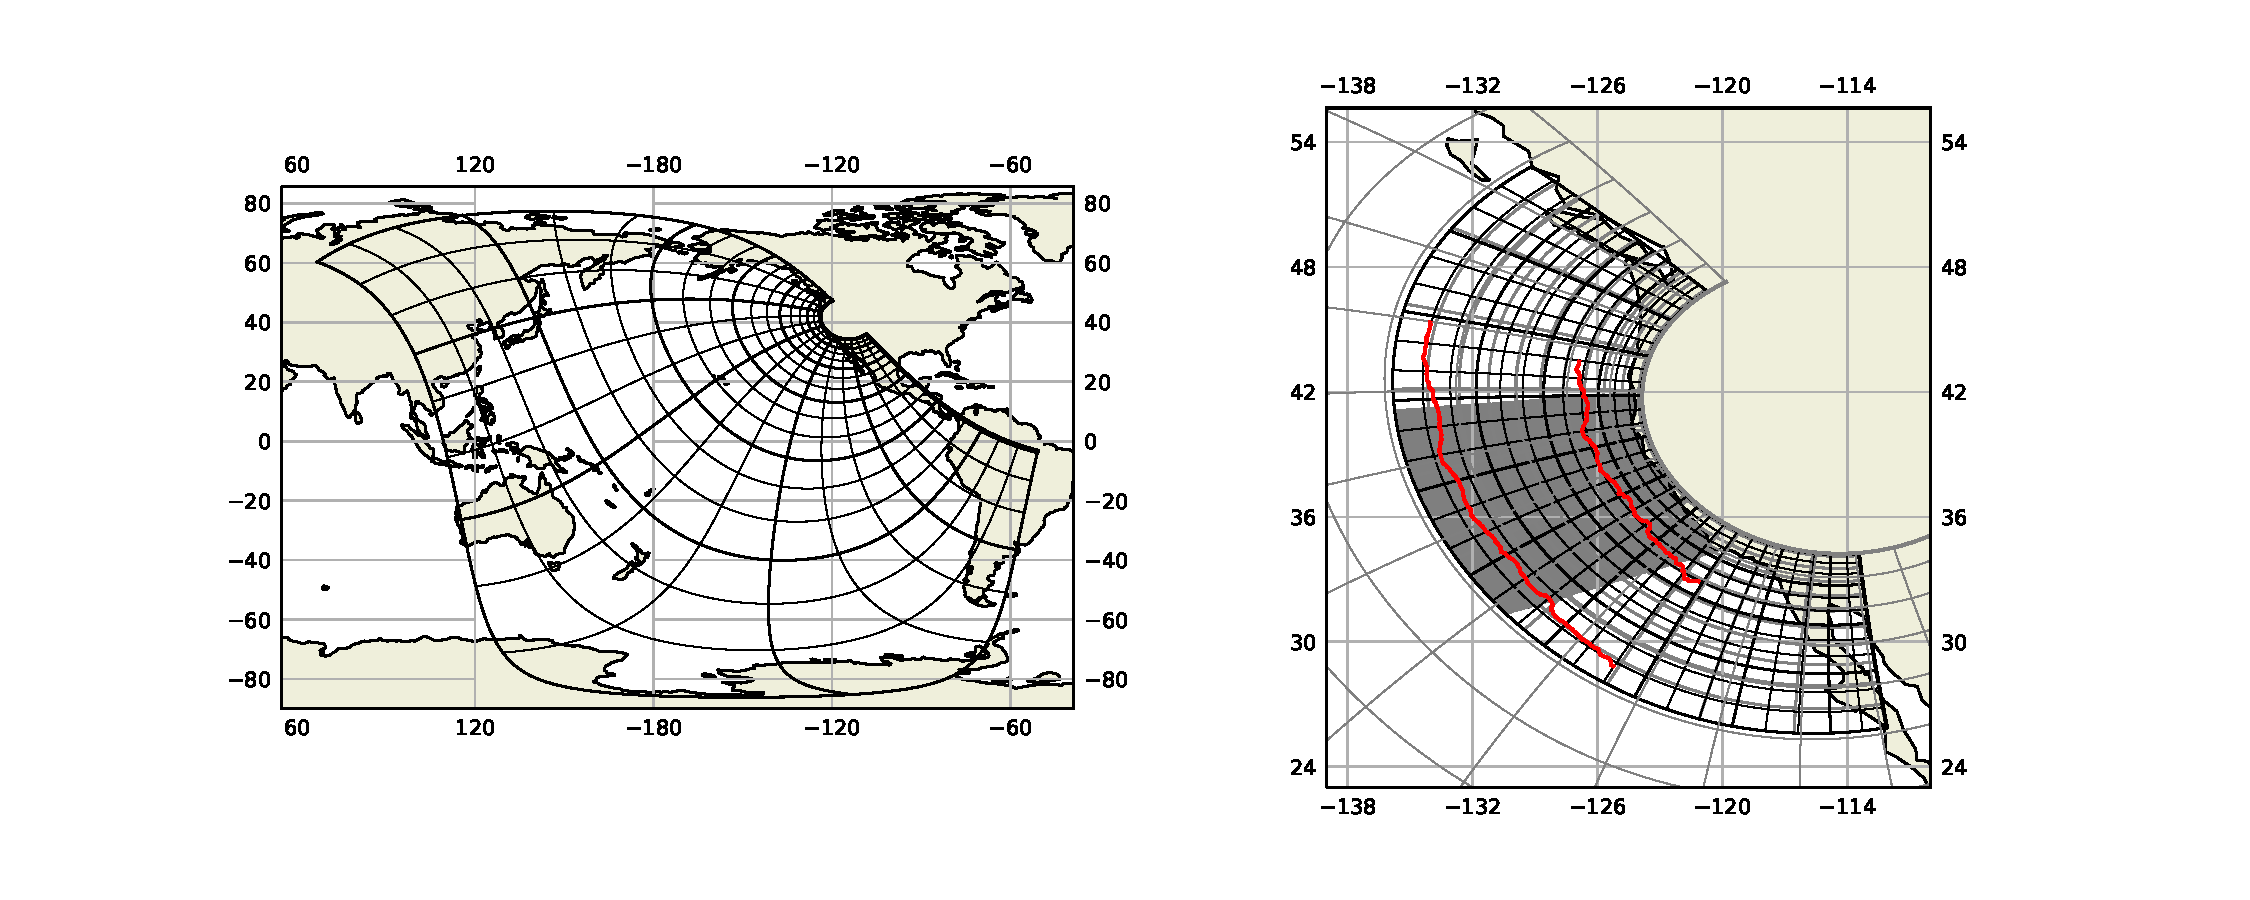
\includegraphics[width=15cm, trim=2cm 0 2cm 0]{../figures/methods_grid.pdf}
    \caption[Horizontal grids]{\textbf{Horizontal grids} for \ac{mr} (left) and HR (right). Red lines denote 200km and $\SI{800}{\kilo\metre}$ distance to coast. The gray area is the analysis domain.}\label{fig:methods-grid}
\end{figure}

\subsubsection{High-resolution model}

The horizontal grid used in the \ac{hr} is also telescopic with the same poles as in \ac{mr}. The horizontal resolution is increased by a factor of $2.5$ to a mean resolution of $\SI{2.8}{\kilo\metre}$ (ranging from $\SI{1.8}{\kilo\metre}$ to $\SI{4.2}{\kilo\metre}$) resulting in a nominal resolution of $\SI{5}{\kilo\metre}$\footref{fn:nominal-resolution}.\\
In contrast to \ac{mr}, \ac{hr} is not integrated on the whole basin. Instead, the grid is clipped at $\around\SI{1000}{\kilo\metre}$ off the coast (see \autoref{fig:methods-grid}) and the results of \ac{mr} are used as lateral boundary conditions. The initial conditions and the atmospheric forcing are the same as for \ac{mr} (interpolated to \ac{hr} grid). The timestep is reduced to $\SI{200}{\second}$.

\section{Mesoscale Eddy Detection}\label{sec:data-methods-eddydetection}

Mesoscale eddies are detected using the algorithm of \textcite{faghmous-2015} with adaptions for curvilinear grids implemented by \textcite{lovecchio-2018-faghmous-adaption}. The algorithm defines an eddy as the largest closed contour of \ac{ssh} anomaly around a single local extreme (minimum for cyclones, maximum for anticyclones). In a first step, local extremes are identified by comparing each pixel to its 5x5 neighborhood. Afterwards, the eddy extent is iteratively constructed around each extreme. At each iteration, neighbouring pixels with a \ac{ssh} value above (or below) a threshold are assigned to the eddy and the threshold is increased (or decreased). The threshold starts from the extreme itself. As soon as the eddy comprises another extreme, the iteration stops and the previous iteration result is used as eddy extent \autocite[see their Figure 1.2]{faghmous-2015}. In this study, the threshold was changed by $\SI{5}{\centi\metre}$ at each iteration.\\
\\
After eddies have been detected in each frame, a tracking algorithm developed by \textcite{chelton-2011} assemble the instances to tracks. The algorithm matches an eddy at time $t$ to an eddy at $t-1$ if it is within a given radius of the previous detection. The radius is based on the propagation speed. In addition, the amplitude and size of the two instances have to be similar, meaning that they do not change more than by a factor of $0.25$ to $2.75$ between $t-1$ and $t$. If no matching eddy was found in $t$, a \textit{fake eddy} with the same size and amplitude as in $t-1$ is placed along the eddy trajectory in $t$ (based on the propagation speed from $t-1$). The fake eddy can be matched in the following time step. This allows missing detections in tracks. The maximum number of consecutive fake eddies can be specified as a parameter \autocite[see their Figure 2]{faghmous-2015}. For this study, the number of consecutive fake eddies is set to $1$ which corresponds to $\SI{2}{\day}$.\\
\\
As proposed by \textcite{faghmous-2015}, the tracks are filtered based on their lifetime. Hence, only eddies belonging to tracks with a lifetime of more than $\SI{4}{\day}$ (corresponding to 2 frames) are considered in this study.

\section{Metrics of Mesoscale Eddy Characterization}\label{sec:data-methods-eddymetrics}

The radius of an eddy $r_e$ is defined as the radius of a circle with the same area as the eddy and is given as
\begin{align}
    r_e = \sqrt{\frac{A_e}{\pi}}
\end{align}
with $A_e$ being the area of the eddy. It is commonly used (e.g. in \textcite{chelton-2011, kurian-2011-eddy-props}) because it is comparable to the Rossby deformation radius.\\
\\
Eddies are associated with temperature and density anomalies. The anomaly of an observable $X$ is given as $X'(t) = X(t) - \overline{X}(t)$ with $\overline{X}$ being the mean state. For a characterization of eddies, $\overline{X}$ should average out all eddy-induced variability but keep variability of larger scales (e.g. seasonal cycle or large-scale gradients). In this study, $\overline{X}(t)$ is approximated by averaging the climatology of $X$ over 60 days around the day of year (DOY, given by $t$) with triangular weighting. The climatology at a given DOY is the average of all snapshots belonging to this DOY.\\
\\
The \ac{eke} is the kinetic energy of mesoscale horizontal motions \autocite{rieck-2019-thesis-eke}. It is given as
\begin{align}
    \text{EKE} = \frac{1}{2}u'v' = \frac{1}{2}(u - \overline{u})(v - \overline{v})
\end{align}
with $u, v$ being the surface horizontal velocity components and $\overline{u}, \overline{v}$ their mean state.\\
\\
Eddy composites are averages of a property (e.g. temperature anomalies) in the eddy impact region over many eddy instances. They can be thought of as a \textit{mean eddy} \autocite{mcgilli-2016-meso-review}. In order to calculate the composites, the eddy instances have to be resized to the same grid. This is achieved by applying the following steps to each eddy instance
\begin{enumerate}
    \item determine radius $r_e$ and center $c_e$ of the eddy
    \item get the data of the target property inside a bounding box of length $n ∗ r_e$ centered at $c_e$
    \item interpolate the extracted data to a fixed grid size of $50\text{px} \times 50\text{px}$.
\end{enumerate}
$n$ determines the eddy impact area and is chosen to be $n = 4$ in this study. In order to perform a meaningful interpolation, only eddies with $r_e > \SI{35}{\kilo\metre}$ are considered for composites in this study.

\section{Detection Algorithm for Submesoscale Fronts}\label{sec:data-methods-submdet}

Submesoscale fronts occur as elongated fronts of strong vertical velocities in the upper ocean \autocite{mcwilliams-2016-subm-currents}. In the course of this study, a detection algorithm was developed which detects fronts in the vertical velocity field. It makes use of three characteristics of the fronts: (1) enhanced vertical velocity (up or down), (2) elongation and (3) consistency in depth. The algorithm consists of three steps which are defined below for the detection of upward fronts (for downward fronts only the sign in the thresholding step changes). The steps are also illustrated in \autoref{fig:methods-submdetection}.\\
\begin{figure}[h]
    \centering
    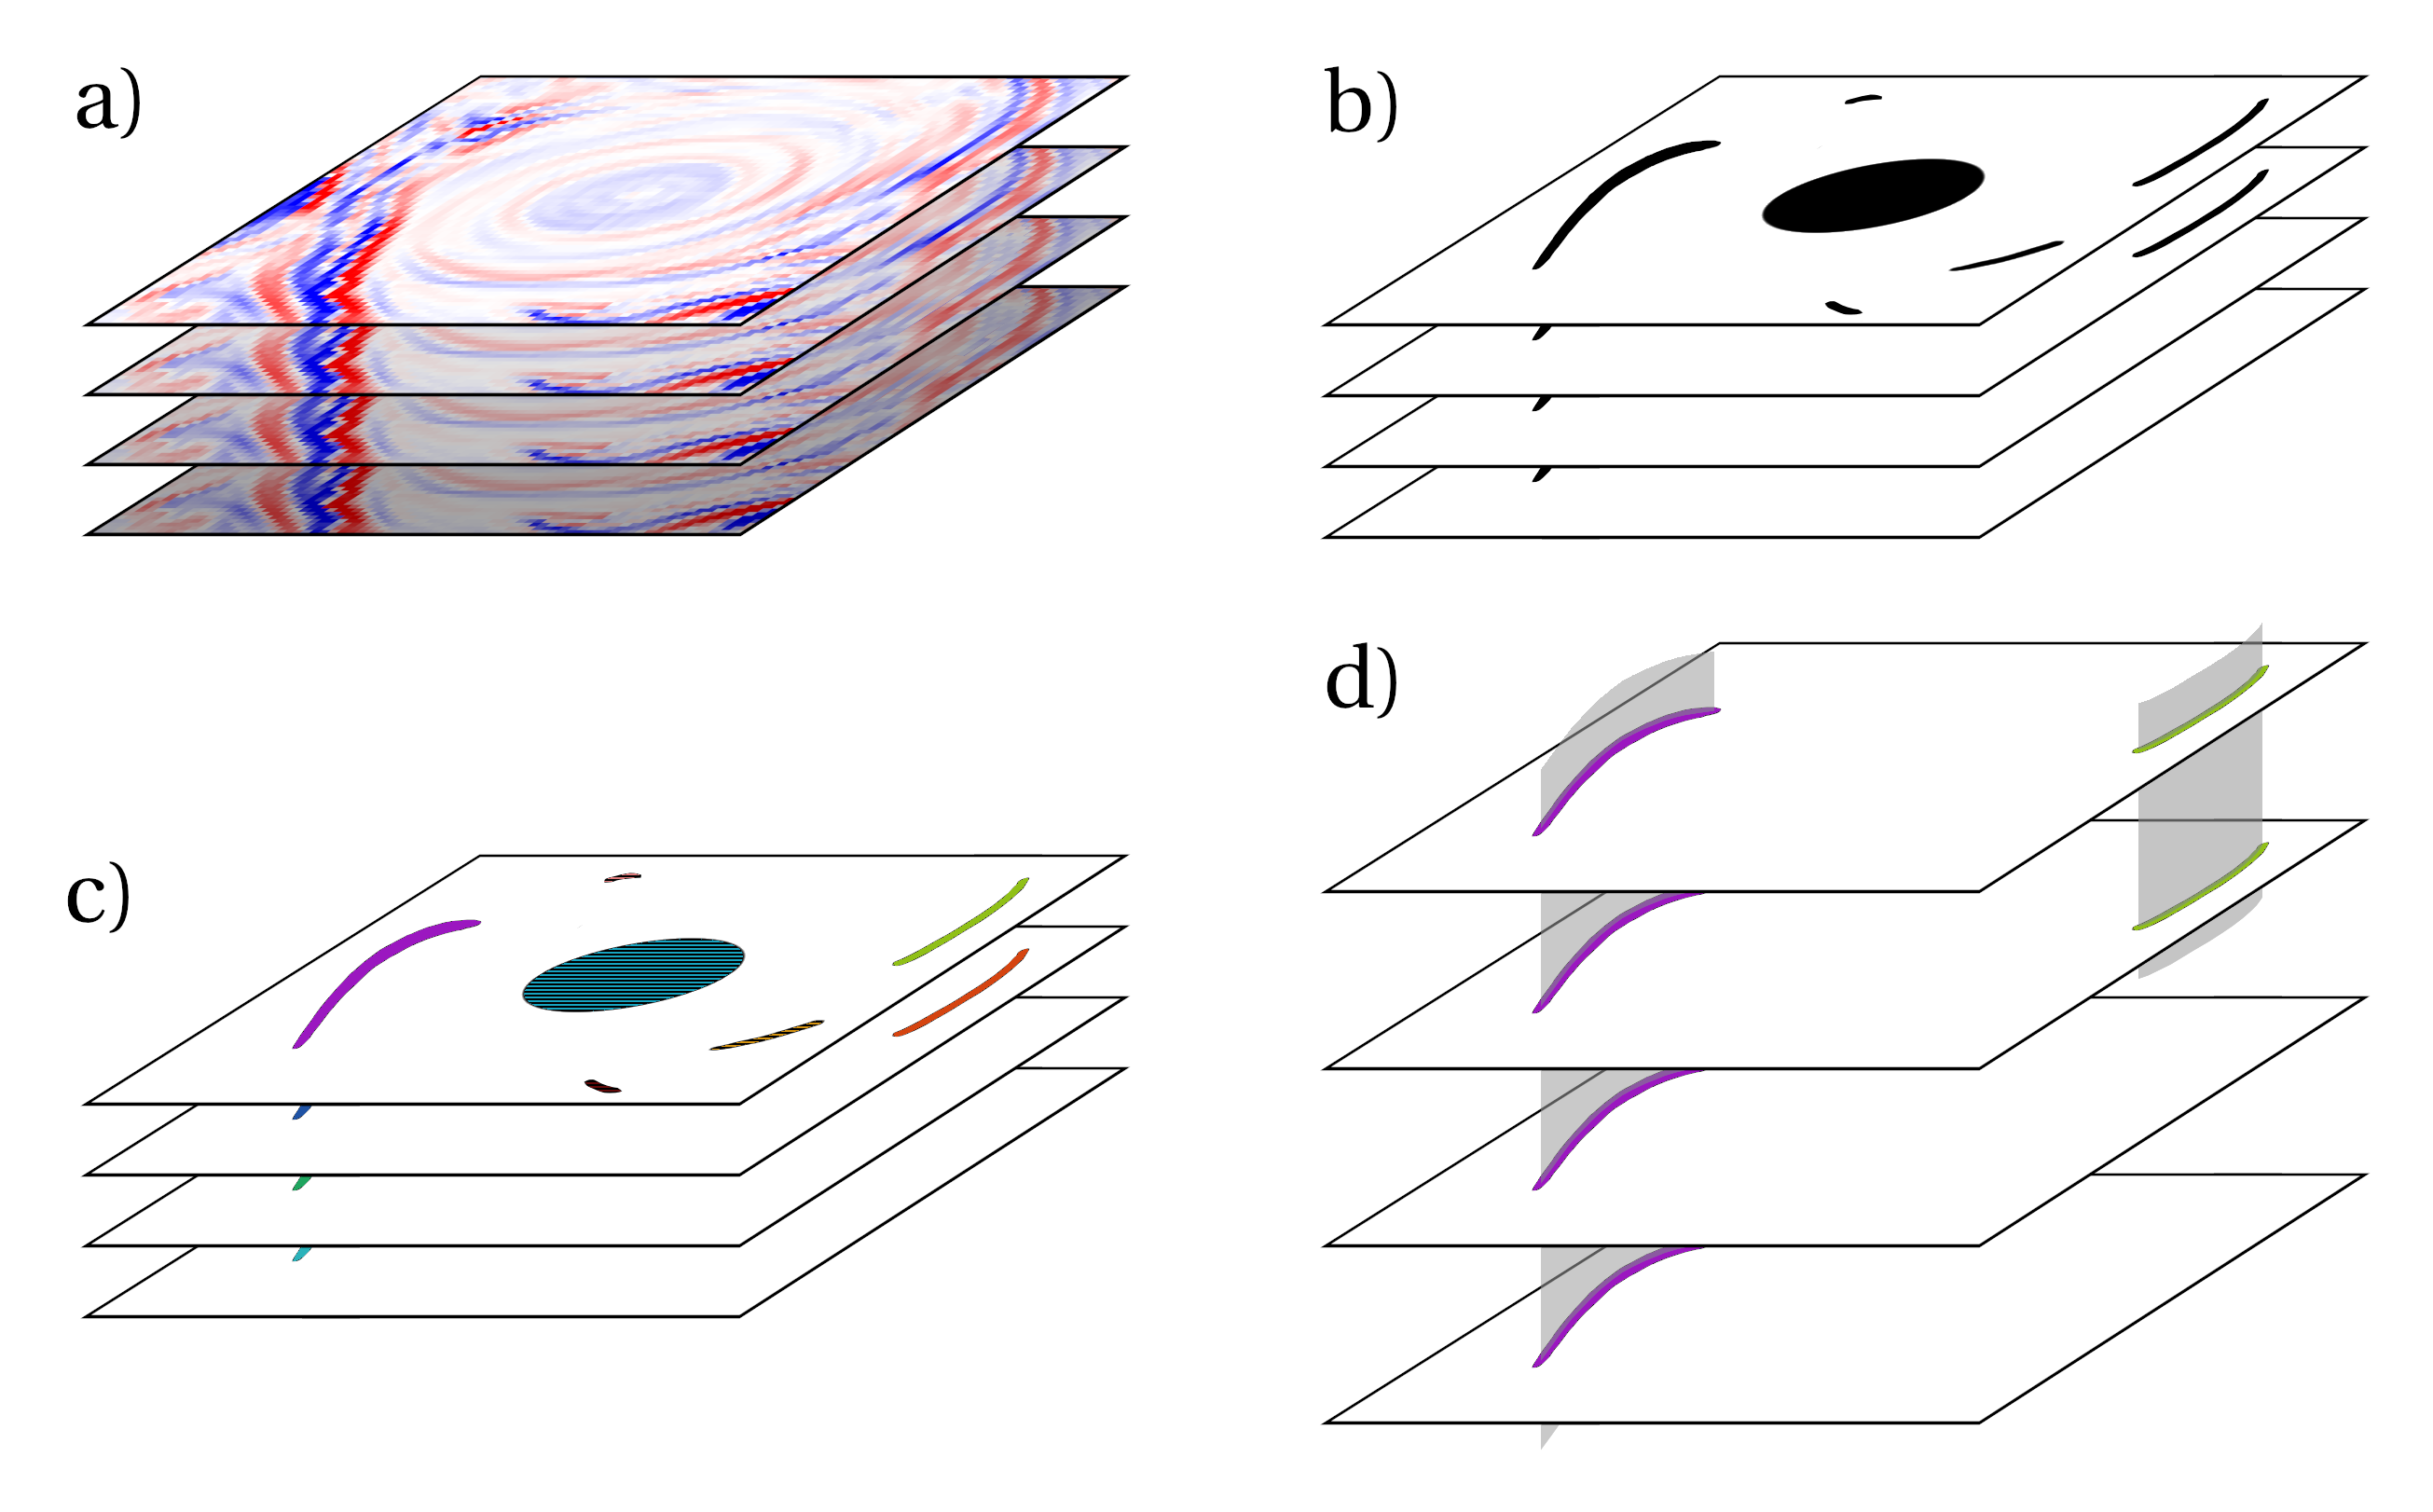
\includegraphics[width=12cm, trim=0 0 0 0]{../figures/subm_algorithm.png}
    \caption[Steps of submesoscale front detection algorithm]{\textbf{Steps of submesoscale front detection algorithm}. (a): The 3D vertical velocity field used as input. (b): Pixels of strong vertical velocities are identified by applying an adaptive threshold $t_w(z)$ ($\Rightarrow P_\text{hvv}$). (c): The pixels are grouped by a 2D connected component analysis to distinct components ($\Rightarrow \widetilde{C}$). Too small or circular components are dropped ($\Rightarrow C$). (d) The remaining components are combined vertically by a 3D connected component analysis to a set of possible fronts ($\Rightarrow \widetilde{F}$). Only fronts that exceed several depth levels are kept ($\Rightarrow F$).}\label{fig:methods-submdetection}
\end{figure}
\\
\\
\\
\textit{Step 1}: A threshold $t_w(z)$ for the vertical velocity is calculated to obtain regions with strong vertical velocities. To this end, the vertical velocity field $w(x, y, z)$ is smoothed laterally (Gaussian filter with $\sigma_\text{lat}$) resulting in $w_\text{smooth}(x, y, z)$. $t_w(z)$ is then calculated as the lateral average of the absolute value of $w_\text{smooth}$:
\begin{align}
    t_w(z) = <|w_\text{smooth}(\cdot, \cdot, z)|>.
\end{align}
Note, that $t_w(z)$ can be different for different depth levels. With $t_w(z)$ a set of pixels with enhanced vertical velocity can be defined for every depth level. This is given as
\begin{align}
    P_\text{hvv}(z) = \left\{p | p \in P(z), w(x_p, y_p, z) - w_\text{smooth}(x_p, y_p, z) \ge 2 t_w(z)\right\}
\end{align}
with $(x_p, y_p)$ being the location of the pixel $p$ and $P(z)$ the set of all pixels at depth level $z$. For downward fronts, the set is given as
\begin{align}
    P_\text{hvv}(z) = \left\{p | p \in P(z), w(x_p, y_p, z) - w_\text{smooth}(x_p, y_p, z) \le -2 t_w(z)\right\}.
\end{align}
\textit{Step 2}: A two-dimensional connected component analysis is carried out on $P_\text{hvv}(z)$ (more precisely on a boolean map where all pixels $\in P_\text{hvv}(z)$ are 1 and all others are 0). This transforms the pixel space into distinct components. The resulting components $\widetilde{C}(z)$ are filtered by two criteria. The first criterion is that the number of pixels belonging to a component $c \in \widetilde{C}$ (denoted as $\#c$) exceeds a minimum threshold of $n_\text{comp}$ pixels. This removes very small components which are considered to be noise. The second criterion is that the ratio between $\#c$ and the area of the bounding box enclosing the component (denoted as $\text{bbox}(c)$) should be smaller than a threshold $r_\text{comp}$ ($0 \le r_\text{comp} \le 1$). This criterion ensures that the components are elongated (a line has a very small ratio, a circle has a ratio of $0.79$). The filtering of $\widetilde{C}(z)$ results in
\begin{align}
    C(z) = \left\{c | c \in \widetilde{C}(z), \#c \ge n_\text{comp}, \frac{\#c}{\text{bbox}(c)} \le r_\text{comp}\right\}
\end{align}
\\
\textit{Step 3}: The identified components are combined vertically. To this end, a set of pixels presumably associated with fronts is constructed:
\begin{align}
    P_\text{front} = \left\{p | p \in \bigcup_{z \in \{0, ..., Z\}} \bigcup_{c \in C(z)}c\right\}
\end{align}
with $Z$ being the maximum depth level. A three-dimensional connected component analysis is carried out on $P_\text{front}$ (as described before) resulting in a set of possible fronts $\widetilde{F}$. A front $f \in \widetilde{F}$ is accepted as a front if its vertical extension (number of depth levels with non-zero components, denoted as $\#_zf$) exceeds a minimum threshold of $n_\text{depth}$ depth levels. This criterion ensures consistency in depth. The final set of detected fronts $F$ is then given as
\begin{align}
    F = \left\{f|f \in \widetilde{F}, \#_zf \ge n_\text{depth}\right\}
\end{align}
\\
\\
The optimal set of parameters was determined by visual inspection of the detection results. The chosen parameters used in this study can be found in \autoref{tbl:subm-detection-parameters}. It turned out that $\sigma_\text{lat}$ is the most important parameter. Because the thresholding step uses the deviation from $w_\text{smooth}$, $\sigma_\text{lat}$ implicitly determines the width and number of detected fronts. This can be seen in \autoref{fig:subm_det_sigma} which shows detections for different values of $\sigma_\text{lat}$. The sensitivity to $\sigma_\text{lat}$ is a strong limitation and future studies should seek a more robust thresholding. In contrast, the results seem to be less sensitive to the choice of $n_\text{comp}$ and $n_\text{depth}$ as small values for these thresholds are sufficient to filter out false detections. Also $r_\text{comp}$ allows for a large margin because most features are strongly elongated and are clearly distinguishable from circular features.\\
\\
Overall, the algorithm shows an acceptable performance. Fronts are detected in both models during winter (see \autoref{fig:subm_det_winter} to \ref{fig:subm_det_winter3} for \ac{hr} and \autoref{fig:subm_det_winter_meso} to \ref{fig:subm_det_winter_meso2} for \ac{mr}) and hardly any fronts are detected during summer (see \autoref{fig:subm_det_summer}). The number of fronts does not seem to be a meaningful metric, because the algorithm detects each upwelling- and downwelling component as a single front. Visual inspection confirms however, that the area covered by submesoscale fronts is captured quite well by the detection algorithm.\\
\begin{table}
    \centering
    \begin{tabular}{l l l l l}
        \toprule
        \textbf{Model} &
        $\sigma_\text{lat}$ &
        $n_\text{comp}$ &
        $r_\text{comp}$ &
        $n_\text{depth}$ \\
        \midrule
        \ac{mr} & 2 & 4 & 0.5 & 5 \\
        \ac{hr} & 2 & 10 & 0.5 & 5 \\
        \bottomrule
    \end{tabular}
    \caption[Parameters for submesoscale front detection]{\textbf{Parameters for submesoscale front detection}}\label{tbl:subm-detection-parameters}
\end{table}

\section{Error Estimation}

The results of this study are based on detections of mesoscale eddies and submesoscale fronts. Unfortunately, the detection algorithms do not provide information about confidence of a detection. Therefore, the uncertainty $\Delta x$ of a value $x$ is approximated in this study by the interannual range of $x$, i.e. $\Delta x = \frac{1}{2}(\text{max}_\text{years}(x) - \text{min}_\text{years}(x))$. Although this approximation is convenient, it is likely to underestimate the true uncertainty because a normal year forcing is used in this study. Moreover, spatial and seasonal variability is not captured by this approach. Hence, the reported uncertainties have to be taken with caution.